%================================================================================
% Implicit Solvent Parametrisation by Force Matching
% Jens Kleinjung and Franca Fraternali
% ISMB 2016 Orlando
% poster
%================================================================================

\documentclass{beamer}
\usepackage[orientation=portrait,size=a0,scale=1.4,debug]{beamerposter}
\mode<presentation>{\usetheme{FC}}
\usepackage{caption}
\usepackage[utf8]{inputenc}
\usepackage[english]{babel}
\usepackage{siunitx} %pretty measurement unit rendering
\usepackage{hyperref} %enable hyperlink for urls
\usepackage{ragged2e}
\usepackage{calc}
\newlength{\mylength}
\usepackage{array,booktabs,tabularx}
\newcolumntype{Z}{>{\centering\arraybackslash}X} % centered tabularx columns
\newcommand{\sig}{$\sigma_i^{SASA}$}
\captionsetup[table]{name=Eq.}
%______________________________________________________________________________
\title{\huge Implicit Solvent Parametrisation by Force Matching}
\author{Jens Kleinjung and Franca Fraternali}
\institute[]{The Francis Crick Institute, King's College London}
\date{\today}
\newlength{\columnheight}
\setlength{\columnheight}{105cm}
%______________________________________________________________________________
\begin{document}
\begin{frame}
\begin{columns}
\begin{column}{.43\textwidth}
\begin{beamercolorbox}[center]{postercolumn}
\begin{minipage}{.98\textwidth}  % tweaks the width, makes a new \textwidth
\parbox[t][\columnheight]{\textwidth}{ % must be some better way to set the the height, width and textwidth simultaneously
%______________________________________________________________________________
\begin{myblock}{Force Matching}
\begin{figure}
\begin{minipage}{0.43\textwidth}
	\centering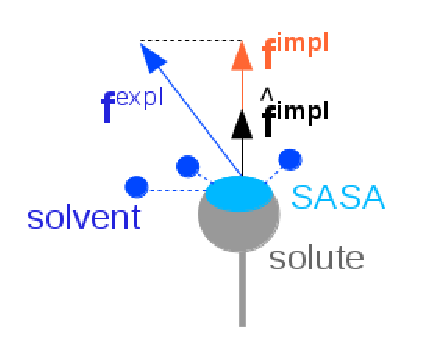
\includegraphics[width=1.0\textwidth]{force_matching1}
	\caption{Force matching: Explicit solvent forces (blue arrow) exerted on the solute are projected on the normal of its SASA (black arrow), yielding the implicit solvent force (orange arrow).}
\label{fig:projection}
\end{minipage}
%______________________________________
\begin{minipage}{0.43\textwidth}
\begin{gather}
	\label{eq:sigma}
	\nonumber \quad \\
	\nonumber \left| \mathbf{f}_i^{impl} \right| \; = \; \hat{\mathbf{f}}_i^{impl} \; \cdot \; <\mathbf{f}_i^{expl}> \\
	\nonumber \quad \\
	\nonumber \sigma_i^{SASA} \; = \; - \, \frac{ \frac{ \partial A_i} { \partial \mathbf{r}_i} }
		{\left| \frac{ \partial A_i} { \partial \mathbf{r}_i} \right| ^2 }
			\, \cdot \, <\mathbf{f}_i^{expl}> \\
	\nonumber \quad
\end{gather}
\begin{table}
\caption{Using the concept of force projection shown left,
the expression for \sig combines the observed forces in explicit
solvent with the derivative of the atomic SASA.}
\end{table}
\end{minipage}
\end{figure}
\end{myblock}\vfill
%______________________________________________________________________________
\begin{myblock}{References}
\footnotesize
\bibliographystyle{abbrv}
\bibliography{./poster}
\end{myblock}\vfill
%______________________________________________________________________________
}\end{minipage}
\end{beamercolorbox}
\end{column}
\end{columns}
\end{frame}
\end{document}
%================================================================================

